\documentclass[main.tex]{subfiles}
\begin{document}

\section{Implementing a Bit-Bang'ed SPI Master}

\subsection{Given Code}
Assume the header shown in listing \ref{code:bit-bang-header} is available for use in the bit-banging implementation of SPI. The transceive function should use CPOL = 1, CPHA = 1. 

\lstinputlisting[caption={Bit Bang HAL Header}, label={code:bit-bang-header}]{code/bitbang_spi/bitbang_spi_header.h}

\spoilerline


\subsection{Bit-Banging Basics}
In embedded systems, communication protocols like SPI are typically handled by dedicated hardware peripherals. These peripherals manage the precise timing and fast data transmission required to communicate over physical wires. However, it is also possible to implement these protocols purely in software, a technique commonly known as \textit{bit-banging}. Bit-banging can be useful in the following scenarios:
\begin{itemize}
    \item When a hardware peripheral (ex: SPI/I2C/UART) is unavailable on the microcontroller, usually because it's not supported, or the EE (\textit{Electrical Engineer}) gave the pins a 'creative reassignment' (accidentally routed incorrect pins during schematic capture).
    \item When a custom or non-standard protocol is required, which cannot be supported by existing hardware peripherals.
\end{itemize}

\noindent Bit-banging is usually implemented by manually controlling the individual pins of a microcontroller in software to emulate a hardware peripheral \cite{looi_bitbanging}. While this approach is slower and uses more CPU resources, it provides flexibility for situations where hardware support is limited. Listing \ref{code:bit-bang-square-ex} shows an example of a square wave generator implemented using bit-banging. Note the use of \texttt{delayMicroseconds()} to control the timing of the square wave, which blocks the CPU until the desired time has passed, contributing to the inefficiency of bit-banging.

\lstinputlisting[caption={Bit-Banged Square Wave Implementation}, label={code:bit-bang-square-ex}]{code/bitbang_spi/bitbang_ex.c}

\subsection{SPI Review}
Consider the SPI timing diagram in figure \ref{fig:spi_timing_2}. The SPI protocol consists of 4 signals: MOSI (Master Out Slave In), MISO (Master In Slave Out), SCLK (Serial Clock), and CS (Chip Select). The master device controls the clock signal and selects the device using the CS signal; data is transmitted on MOSI and received on MISO simultaneously on predefined edges of the clock signal.

\begin{figure}[H]
    \centering
    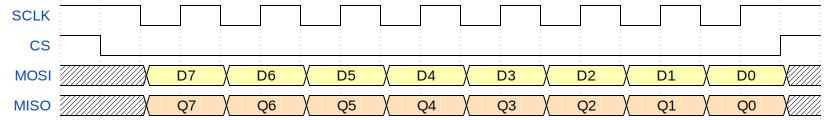
\includegraphics[scale=0.4]{generated_images/svg_generated/spi_waveform.png}
    \caption{1-byte SPI Timing Diagram}
    \label{fig:spi_timing_2}
\end{figure}

\noindent Note that the SPI protocol can be configured in different clock sampling modes, which define the clock polarity (CPOL) and phase (CPHA). Figure \ref{fig:spi_timing} shows CPOL = 1, CPHA = 1. A SPI slave device's datasheet will usually specify the required CPOL and CPHA settings for proper communication real-world implementation.
\begin {itemize}
    \item \textbf{CPOL (Clock Polarity)}: Determines the idle state of the clock signal. CPOL = 0 means the clock is low when idle, while CPOL = 1 means the clock is high when idle.
    \item \textbf{CPHA (Clock Phase)}: Determines when data is sampled and changed. CPHA = 0 means data is sampled on the leading edge (first transition) of the clock, while CPHA = 1 means data is sampled on the trailing edge (second transition) of the clock.
\end{itemize}

\subsection{Bit-banging SPI Implementation}
Going through the timing diagram in figure \ref{fig:spi_timing} piece by piece, we can implement the SPI protocol in software. The key parts are as follows:
\begin{itemize}
    \item Pull the CS line low to select the slave device. Wait for a brief period (referred to as \textit{setup time}).
    \item Generate a square wave on the SCLK line, ensuring the correct CPOL and CPHA settings.
    \item Loop through each bit of the tx byte starting from the most significant bit (MSB), and transmit the logical value of the bit on the MOSI line on every SCLK falling edge.
    \item In parallel, read the MISO line on the rising edge of SCLK line to receive the slave's response, and write it to the corresponding bit in the received byte buffer. 
    \item Repeat for the specified number of bytes.
    \item Terminate the SPI transaction by pulling the CS and SCLK line high to deselect the slave device.
\end{itemize}

\noindent Listing \ref{code:bit-bang-spi} shows a basic implementation of a bit-banged SPI master transceive.

% TODO: Make sure we talk about bit shifting somewhere... it's kind of a fundamental topic lol

\lstinputlisting[caption={Bit Bang SPI Implementation}, label={code:bit-bang-spi}]{code/bitbang_spi/bitbang_spi.c}

\end{document}
